% !TEX root = ../Dokumentation.tex
\subsection{Antrieb}
\textbf{Funktionsbeschrieb}\\[0.2cm]
Als Antrieb wird ein DC-Getriebemotor verwendet, der an der Unterseite montiert wird und für die Vor- sowie Rückwärtsbewegungen des Fahrzeugs zuständig ist.
Die aktuelle Drehzahl des Motors wird von einem Encoder erfasst. Dieser wiederum sendet die gemessenen Daten an den Mikrocontroller der schlussendlich die Anzahl Umdrehungen reguliert.\\[0.2cm]
\textbf{Komponentenbeschrieb}
\begin{figure}[H]
\centering
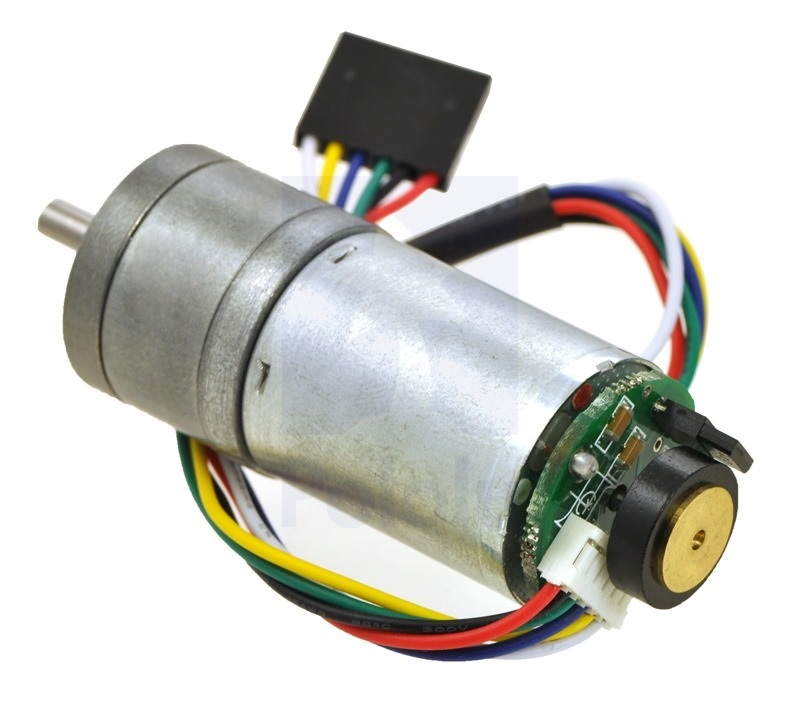
\includegraphics[width=0.5\textwidth]{03_Loesungskonzept/pictures/Antrieb_Encoder.jpg}
\caption{DC-Motor mit integriertem Encoder (Quelle:http://https://www.pololu.com/product/3217)}	
\end{figure}
Gewählt wurde ein Hochleistungsgetriebemotor von Pololu
Die technischen Daten sind folgende:
\begin{itemize}
\item Leerlaufstrom: 0.3 A
\item Leerlauf-Drehzahl: 210 U/min
\item Betriebsspannung: 12 V DC
\item Spitzendrehmoment: 1.16 Nm
\item Max. Laststrom: 0.5 A
\end{itemize}
\textbf{Begründung}\\[0.2cm]
Der ausgewählte Motor punktet vor allem aufgrund seiner kleinen und kompakten Bauform. Da der Montageort für den Antrieb am Fahrzeug nicht verändert werden kann, ohne umständliche Wellen zu installieren, ist die Baugrösse relativ beschränkt.
Ein weiterer Punkt ist, dass er sich als Gleichstrommotor leicht ansteuern lässt und damit die Handhabung vereinfacht.Ausschlaggebend war aber das er bereits einen integrierten Encoder besitz.\\[0.2cm]
\textbf{Vergleich Konzept und Umsetzung}\\[0.2cm]
Im Pren1 viel die Wahl auf einen anderen DC-Motoren der von der Schule zur verfügung gestellt wurde. Da dieser aber keine interne Regelung besass, wurde geplant einen separaten Encoder zu beschaffen der die Drehzahl des Motores reguliert. Jedoch gestaltete sich die Umsetzung als zu aufwändig und daher wurde entschieden einen DC-Motoren mit integriertem Encoder zu verwenden.
\subsubsection{Geschwindigkeitsregelung}
Damit das Fahrzeug mit einer konstanten Geschwindigkeit fahren kann, musste ein Regler eingebaut werden.
\begin{figure}[H]
	\centering
	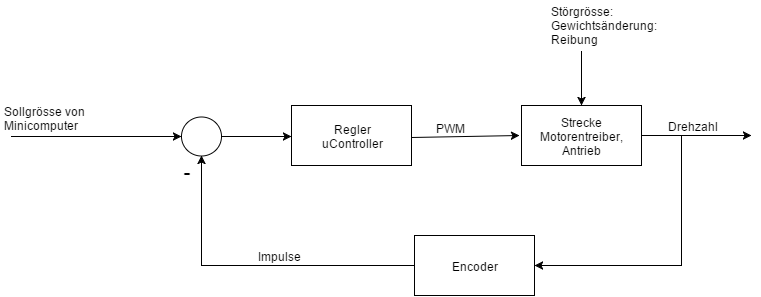
\includegraphics[width=1\textwidth]{03_Loesungskonzept/pictures/Gesch_Regelung.png}
	\label{Regelung_Gesch}
	\caption{Grober Antriebsregelkreis}
\end{figure}
Hier ist der unveränderte Regelkreis aus Pren1 zu sehen.\\Für die Geschwindigkeitsregelung wurde ein PID-Regler verwendet. Damit die Parameter für die Geschwindigkeitsregelung richtig eingestellt sind, wurde die Schrittantwort des DC-Motors per Encoder ausgemessen. Die Schrittantwort von Null auf volle Geschwindigkeit (210RPM) sieht ungefähr so aus:
\begin{figure}[H]%Position festigen
\centering
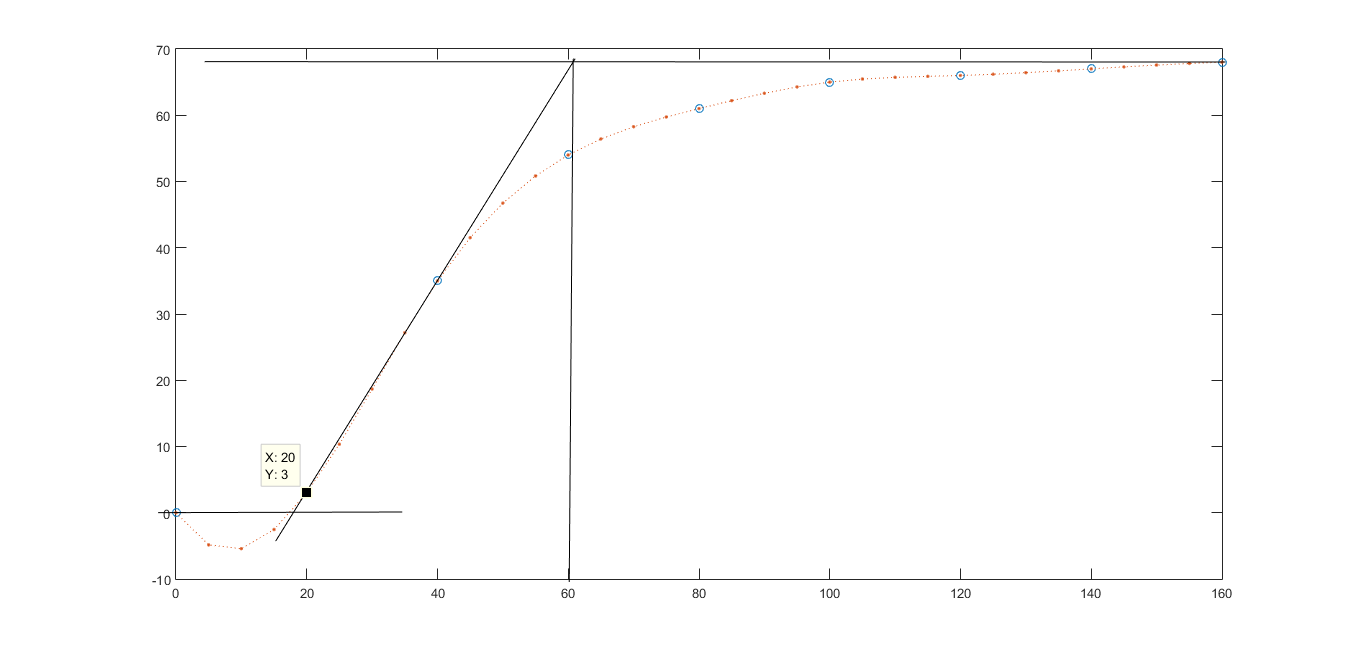
\includegraphics[width=0.9\textwidth]{03_Loesungskonzept/pictures/Sprungantwort.png}
\caption{Die Schrittantwort des DC-Motor im Matlab}
\label{fig:schrittantwort}
\end{figure}
Daraus konnten die Konstanten Tg=63ms und Tu=17ms ausgelesen werden(Einführung in die Regeltechnick S.71). Nach den Einstellregeln nach Chien-Hrones-Reswick konnten die Konstanten Tn, Tv und Kp berechnet werden(Einführung in die Regeltechnick S.215). Daraus ergaben sich die Werte Kp1=2.22, Tn=0.063, Tv=0.0085.
Diese Werte sind jedoch für kontinuierliche Regler und nicht wie in diesem Fall für diskrete Regler. Damit die Werte korrekt sind, mussten die Werte noch weiter verrechnet werden.(Einführung in die Regeltechnick S.247)
\[ T=Abtastperiodendauer=50ms\]
\[ Kp=Kp1*32=2.22*32=72\]
\[ Ki=Kp1*32*T/(2*Tn)=2.22*32*0.05/(2*0.063)=28\]
\[ Kd=Kp1*32*2*Tv/T=2.22*32*2*0.0085/0.05=5.44 =>5\]
Diese Werte sind die Regelparameter. Die Multiplikation mit 32 ergibt sich dem Grund, dass auf dem Mikrocontroller nicht mit Fließkommazahlen gerechnet wird. Somit werden die Werte bei den Parameter hochskaliert und später nach der Verrechnug mit der Regelabweichung wieder dividiert.
Diese Parameter wurden programmiert und ausgemessen. Ein Sollgeschwindigkeit von 150mm/s wurde dem Regler vorgegeben (entspricht einem Encoderwert von 108)
\begin{figure}[H]%Position festigen
\centering
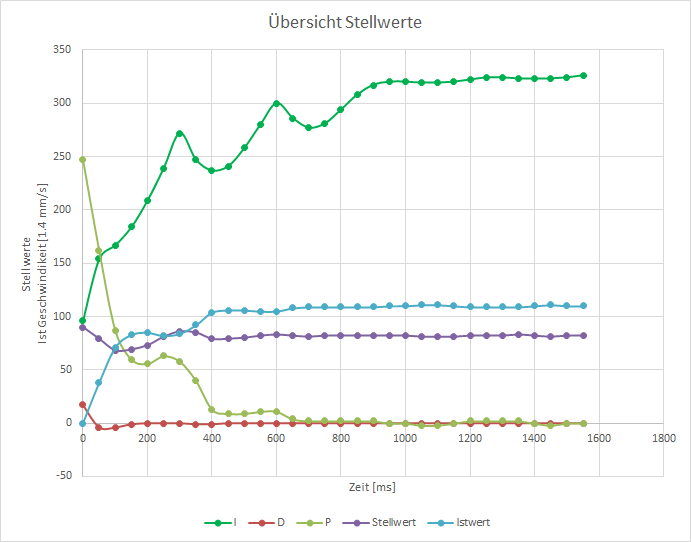
\includegraphics[width=0.9\textwidth]{03_Loesungskonzept/pictures/StellwertePID.png}
\caption{Die Istwert verglichen mit dem Stellwert}
\label{fig:IstSollwertVergleich}
\end{figure}
Hier zeigt sich, dass der Regler nicht Perfekt eingestellt ist, jedoch nach einer halben Sekunden den Sollwert erreicht hat. Dies ist für unsere Anwendung ausreichend und wurde deshalb so belassen.\\[0.2cm]
\textbf{Vergleich Konzept und Umsetzung}\\[0.2cm]
Die Geschwindigkeitsregelung wurde genau so implementiert, wie es im Pren1 geplant war.
\subsubsection{Encoder}
Damit die Drehzahl des Motors ermittelt werden kann, braucht es einen Encoder. Dieser wurde mit dem Antriebsmotor mitgeliefert. Dies war sehr nützlich, da somit keine eigene aufwändige Lösung nötig war. Der Encoder muss mit 5V gespiesen werden. Als Ausgang hat der Encoder zwei Signale. Hier sind diese zu sehen:
\ref{fig:encoder_out}
\begin{figure}[H]%Position festigen
\centering
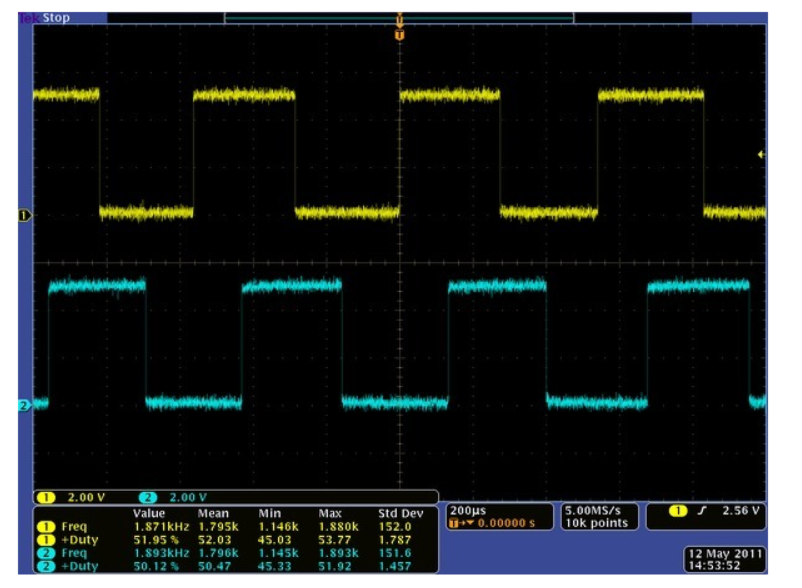
\includegraphics[width=0.6\textwidth]{03_Loesungskonzept/pictures/Encoder_Out.png}
\caption{Beispiels Ausgangssignal des Encoders (Quelle:pololu.com)}
\label{fig:encoder_out}
\end{figure}
Mit Hilfe dieser beiden Signalen gibt es 48 Ticks pro Umdrehung des Motors (ohne Übersetzung). Damit sind es 48Ticks/Umdrehung * 47 (Übersetzung) = 2'256 Ticks pro tatsächlicher Motorenumdrehung. Dies ergäbe eine Genauigkeit von 0.027mm/Tick bei unserem Fahrzeug. Dies ist sehr viel, darum wurde entschieden nur ein Signal auszuwerten. Damit ergibt sich eine Genauigkeit von 0.05mm/Tick. Dies ist immer noch sehr präzise.
Die Auswertung des Signales geschieht im Mikrocontroller. Das Encodersiganl wird über einen Spannungsteiler auf einen Pin des Freedomboard geführt. Diese löst bei jeder Flankenänderung einen Interrupt aus. Im Interrupt wird einfach einen Zähler hochgezählt. Dieser Zähler wird alle 40ms ausgelesen und wieder auf Null gesetzt. Der ausgelesene Wert ist der Ausgangswert des Encoders. Bei voller Geschwindigkeit beträgt dieser Wert Beispielsweise 140 und bei halber Geschwindigkeit 70.\\[0.2cm]
\textbf{Vergleich Konzept und Umsetzung}\\[0.2cm]
Im Konzept war ebenfalls ein Encoder eingeplant. Jedoch war Ende Pren1 noch nicht klar definiert, wie dieser wirklich realisiert werden sollte. Eine eigene Lösung über eine Lichtschranke wurde in Betracht gezogen. Anfangs Pren2 wurde wurde dieses Konzept nochmals überdacht. Da sowieso ein neuer Motor eingesetzt werden sollte, wurde entschieden einen Motor zu wählen, welcher bereits einen Encoder "intergriet" hatte. Diese Lösung ist weniger aufwändig, benötigt weniger Platz und ist dennoch kostengünstiger als eine eigene Lösung.\\[0.2cm]
